\documentclass{beamer}
\mode<presentation>
{
  \usetheme{Warsaw}
   \setbeamercovered{transparent}
}
\usepackage{graphicx}
\usepackage[english]{babel}
\usepackage[utf8]{inputenc}
\usepackage{times}
\usepackage{movie15}
\usepackage[T1]{fontenc}
\title[Natural Language Inference system for Computer games]
{Natural Language Inference system for Computer games}

\author[] 
{
\footnotesize
P.~Dineshswamy~~~~~~~~~~~~~~~~~~~~~~21909104023\\
A.~GaneshSubramanian~~~~~~~~~21909104026\\
}
\institute[Sri Venkateswara College of Engineering] 
{
\textbf{Guided By: Dr.V. Vidhya, Phd}\\
Assistant Professor\\
Department of Computer Science and Engineering\\
 Sri Venkateswara College of Engineering
}

\AtBeginSubsection[]
{
  \begin{frame}<beamer>{Outline}
    \tableofcontents[currentsection,currentsubsection]
  \end{frame}
}

\beamerdefaultoverlayspecification{<+->}
\begin{document}
\begin{frame}
  \titlepage
\end{frame}
\begin{frame}{Outline}
  \tableofcontents
\end{frame}
\section{Abstract}
\begin{frame}{Abstract}
\small
\begin{itemize}
\item
To develop a new way of voice interaction with natural language as interface  for  startegy based computer games 
\item
To allow a Game player to control all the NPC(non-playing characters) in the game 
\item
To enable the Game player make strategic decisions based on perceptions recieved from all the NPC(non-playing characters)
\item
To build a game to achieve DDM(Dynamic decision making)
\item
To increase the number of degrees of freedom in gaming environment and to make  rich human  computer interaction
  \end{itemize}
\end{frame}

\section{Introduction}
\begin{frame}{Introduction}
\footnotesize
\begin{itemize}
\item
Computer games are a major recreational activity .The challenge of interaction with the computer games is to transform it more engaging.
\item		
Here, the interaction with the computer game will be via speech recognition . The  recognised speech  will be processed with state of art NLP techniques to infer . The inference is used to decide the next action.The user can communicate with NPC using his natural language .
\item
			eg :\\
					player:"HEY STEP OUTSIDE , WE HAVE AN INCOMING . COPY THAT"\\
					NPC: "I CANT , I SUSPECT THERE IS A MINE FIELD IN FRONT OF ME.COPY THAT"\\
					player:"GOT IT " .\\
 (this updates the knowledge base of characters i.e an update to their map , marking that place as danger)
  \end{itemize}
\end{frame}


\begin{frame}{Traditional game}
\begin{figure}[ht]
\includemovie[poster,text={\small(Loading video...)},autopause]{6cm}{4cm}{example.avi}
\end{figure}
\end{frame}


\section{Existing works}
\subsection{Keyboard and gesture based interaction }
\begin{frame}{Keyboard and gesture based interaction }
\begin{itemize}
\item
A computer game is played by pressing or holding the  key or combination of keys for a while. This key pressing  events are transformed into actions on the computer game. \\ Gesture based interaction , recognises the users gestures via a web-cam or trackpad or any other  sensory devices. The gesture based recognition is then transformed into suitable actions on the game .
\end{itemize}

\end{frame}


\begin{frame}{Keyboard and gesture based interaction }
\textbf{Limitations}

\begin{itemize}
\item
A single player cannot control the whole team . The non playing characters are pre determined.
\end{itemize}

\begin{itemize}
\item			
			The user has to remember complete keycombinations or gestures and need to choose what to do when ? .
\end{itemize}

\begin{itemize}
\item
			The key combinations  vary for different platforms .
\end{itemize}

\begin{itemize}
\item
			A single key combination or gesture  cannot perform a complex action in the game .
\end{itemize}

\begin{itemize}
\item
			Cannot produce illusion of intelligence in the behaviour of non-player characters .
\end{itemize}
\end{frame}
\subsection{Automatic Speech recognition systems }
\begin{frame}{Automatic Speech recognition systems}
\begin{itemize}
\item
Voice driven commands can be used to control the game .\\ The ASR works by converting speech to text and then matching the text against suitable actions .
\end{itemize}
\end{frame}


 \begin{frame}{Automatic Speech recognition systems}
\textbf{Limitations}

\begin{itemize}
\item
Speech recognition systems however, do not support emotions , attitudes, tones etc. 
\end{itemize}

\begin{itemize}
\item			
			Allows only restricted input .
\end{itemize}

\begin{itemize}
\item
			User needs to remember all the key words .
\end{itemize}

\begin{itemize}
\item
			Disruptions in input due to factors like accent/poor performance in input device(mic) .
\end{itemize}

\begin{itemize}
\item
			User cannot give multiple constraints to a NPC .
\end{itemize}
\end{frame}

\section{Solutions to existing problems}
\begin{frame}{Solutions to existing problems}
\small
\begin{itemize}
\item
The game player should play the without any prior knowledge of key-combinations or gestures .
\item
The game player should have control or communication with multiple NPC's .
\item
Achieving complex actions must be feasible .	 
\item
Recognised speech must be transformed into actions via inferences and not just by a mapping between  text and actions .
\end{itemize}
\end{frame}


\section{Proposed Work}
\begin{frame}{Proposed Work}
\small
\begin{itemize}
\item
The player will interact with the game through voice interaction . This speech is in turn converted to sequence of sentences . These sentences are inferred with a state of art nlp techniques for inference and converted into a suitable action .The inference may perform multiple actions from single speech .

\end{itemize}

\end{frame}

\section{Proposed Architecture}
\begin{frame}{Proposed Architecture}
\small
\begin{itemize}
\item
\hspace{2cm}
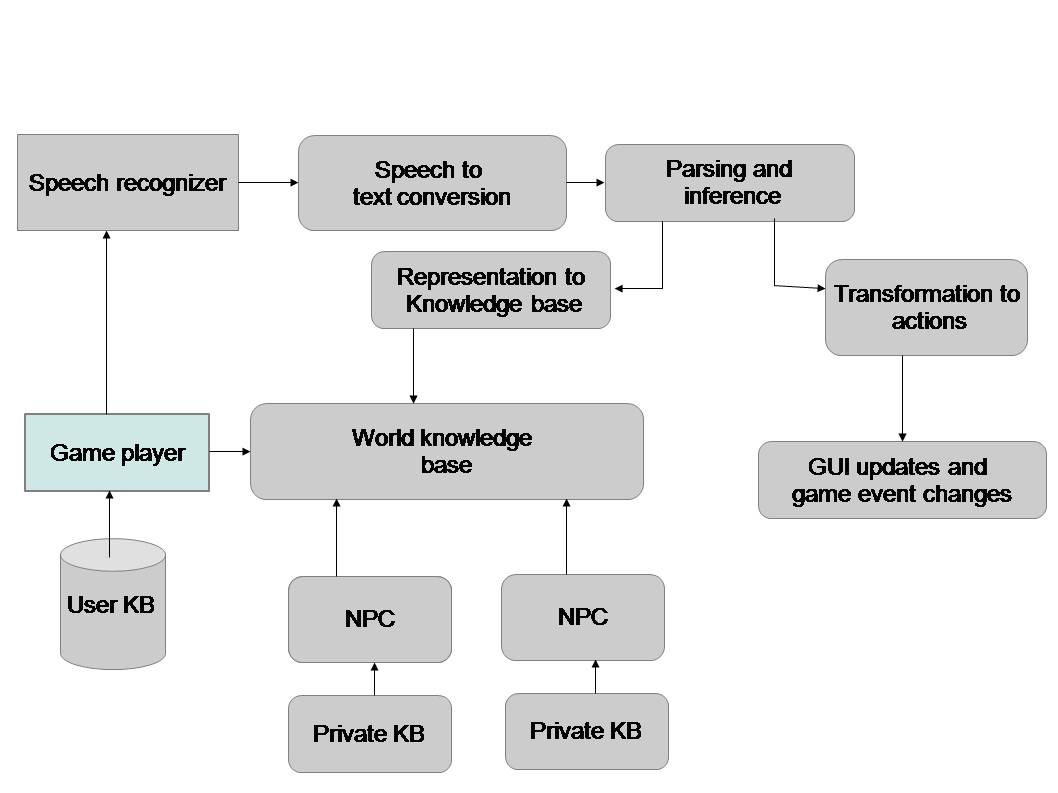
\includegraphics[height=2.1in,width=2.5in]{architecture.jpg}
\end{itemize}

\end{frame}





\section{References}
\begin{frame}{References}
\scriptsize
[1] Moyen Mohammad Mustaquim, “Automatic speech recognition- an approach for designing inclusive games”,Multimedia Tools and Applications, 2011 -Springer
,DOI 10.1007/s11042-011-0918-7\\
\vspace{0.5cm}
[2]Gabsdil, M. (2003). Clarification in spoken dialogue systems. In Proceedings of the 2003 AAAI Spring Symposium. Workshop on Natural Language Generation in Spoken and Written Dialogue (pp. 28-35).\\
\vspace{0.5cm}
[3]Wang, Y. (2010, December). Speech Recognition Applied in Games. In Computational Intelligence and Software Engineering (CiSE), 2010 International Conference on (pp. 1-4). IEEE.\\
\vspace{0.5cm}
[4]Gabsdil, M.; Koller, A.; and Striegnitz, K. 2002. Natural
Language and Inference in a Computer Game. In Proceed-
ings of Coling 2002.
\vspace{0.5cm}
\end{frame}
\begin{frame}
\hfill\LARGE \emph{"If some problem has complex solution , then it must be possible, if a solution is possible then make it simple"}\hspace*{\fill} \\
\hspace{5cm} \textbf{Apple}
\end{frame}



\end{document}


